\documentclass{article}
\usepackage[top=0.2in, bottom=0.1in,left=1.5cm,right=1.5cm]{geometry}
\usepackage{graphicx}
\usepackage{background}

\SetBgScale{1}
\SetBgAngle{0}
\SetBgColor{black}
\SetBgContents{\rule{.5pt}{\paperheight} \rule{.5pt}{\paperheight} 
\qquad \qquad \qquad \qquad \qquad \qquad \qquad \qquad \qquad 
\qquad \qquad \qquad \qquad \qquad \qquad \qquad \qquad \qquad 
\qquad \qquad \qquad \qquad \qquad \qquad \qquad \quad \quad \, \rule{.5pt}{\paperheight} \rule{.5pt}{\paperheight}
}

\begin{document}

\hrule  
\vspace{0.1in}
\includegraphics[width=4cm]{chalk_logo.png}
\huge{ \textbf{CB02 - Switching Power Supply}} 
\vspace{0.05in}
\hrule 
\vspace{0.05in}


\mbox{
\begin{minipage}[t]{0.4\linewidth}
\vspace{0pt}
\large
\textbf{Features and Benefits}
\normalsize
\begin{itemize}
\item Wide input range [5v-24v]
\item High current(1.5A) output
\item Stable 5V output +-2\%.
\item Multiple protection schemes
\item Current and Temperature sense via space saving I2C
\item I2C reports current, voltage, power, and temperature.
\item Alert pin to alert of overcurrent conditions.
\item Soft-startup and current limit.
\item Extreme effeciency of up to 95\%.
\item Low switching frequency of 500kHz.
\item Enable pin disconnects output.
\end{itemize}
\end{minipage}

\vrule
\vspace{0.3in}

\begin{minipage}[t]{0.5\linewidth}
\vspace{0pt}
\large{\textbf{Descritpion}} 
\\

\normalsize
CB02 is a 1.5 amperes step down power supply.  It is a fully contained buck regulator with extremely wide input range and is able to maintain an extremely high efficiency over the whole input range [87-95\%]. In addition, the voltage regulation is extremly stable over rated temperature range. \\
CB02 provides a soft-startup of 2.4 ms, and a current limit of 2 amperes. In addition there is an ENABLE line which allows to completely disconnect the output from the input. This also turns off the internal regulator. The shutdown current is very small [in the mA range].\\
Switching regulato contains a number of protection features such as thermal shutdown, overvoltage and undervoltage reset and current limit. In addition a separate temperature and current sensors are provided on the same I2C bus. The current sensor is intelligent and will provide voltage, current and power, while it is powered from a separate linear regulator. \\
There are also two LEDs providing diagnostic outputs. They are connected to the input and the output voltage line. This allows an easy cursory glance to tell if a power supply is connected and enabled. 

\end{minipage}
} %end mbox
\\
\hspace{0.3in}
\hrule
\hspace{0.3in}
\begin{center} 
\large{\textbf{Typical Application}}
\end{center}
\begin{center}
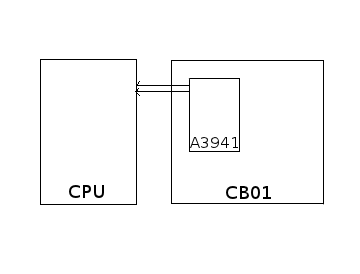
\includegraphics[width=6in]{cb01_typical.png}
\end{center}
\hrule
\newpage
\large{\textbf{Electrical Characterestics}} \\
%page 2!
\begin{center}
\begin{tabular}{|l | l |c| c|c|c|c|}
\hline
Characteristics & Symbol &Test Conditions & Min & Typ & Max & Units \\ \hline
Functional Input Voltage& $V_{in}$& & 5.8&12&24&V \\ \hline 
Output Voltage & $V_{out}$ & Over input voltage& 4.9 & 5.0 & 5.1 & V \\ \hline
Output Current & $I_{max}$ &Output current& 0 & & 1.5 &A \\ \hline
Efficiency & Eff &Vin=12V, Iout=1.5A& & 95 &  & \% \\\hline
\hline
\end{tabular}
\end{center}

\end{document}


